\documentclass[11pt]{article}
\usepackage{hw-solutions-common}
\usepackage{tikz}
\usetikzlibrary{arrows.meta,decorations.markings}

\begin{document}

\hwsolhead{Written HW 8}{Problem statements from Knight, \emph{Physics for Scientists and
Engineers} (5th ed., Global Edition), Chapter 29. $\mu_0 = 4\pi\times10^{-7}\text{
T}\cdot\text{m/A}$ throughout.}

%============================================================
\problem{29.50}{3}{The earth's magnetic dipole moment, $8.0\times10^{22}\
\text{A}\cdot\text{m}^2$, is modeled as arising from current flowing around a
3000-km-diameter loop made from a very fat, 1000-km-diameter ``wire'' of
molten iron (both diameters measured from the wire's centerline). (a) What
current flows in the loop? (b) What is the current density $J$ in the loop?
(c) Compare that to the current density of an ordinary 1.0 A current in a
1.0-mm-diameter wire --- is the earth's current density large or small?}

\model{A current loop's dipole moment is $\mu=IA_{\text{loop}}$, where
$A_{\text{loop}}$ is the area enclosed by the loop's \emph{centerline} ---
that's what fixes the current, regardless of how fat the wire is. Current
\emph{density} is a separate idea: $J=I/A_{\text{wire}}$, the same current
spread over the wire's own cross-sectional area. Here those two areas are
wildly different, since the ``wire'' is nearly as big as the loop itself.}

\visualize{
\begin{center}
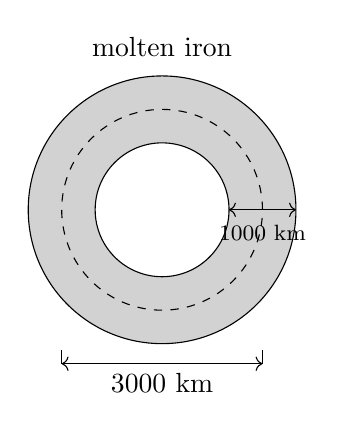
\begin{tikzpicture}[scale=0.85]
\fill[gray!35] (0,0) circle (2.0);
\fill[white] (0,0) circle (1.0);
\draw (0,0) circle (2.0);
\draw (0,0) circle (1.0);
\draw[dashed] (0,0) circle (1.5);
\node[above] at (0,2.15) {molten iron};
\draw[<->] (1.0,0) -- (2.0,0);
\node[below] at (1.5,-0.08) {\footnotesize $1000$ km};
\draw[<->] (-1.5,-2.3) -- (1.5,-2.3);
\node[below] at (0,-2.3) {$3000$ km};
\draw (-1.5,-2.1) -- (-1.5,-2.3);
\draw (1.5,-2.1) -- (1.5,-2.3);
\end{tikzpicture}
\end{center}
The dashed circle is the loop's centerline (radius 1500 km, fixing
$A_{\text{loop}}$); the gray annulus is the wire's own cross section (radius
500 km, fixing $A_{\text{wire}}$).}

\solve{(a)
\[
A_{\text{loop}} = \pi r_{\text{loop}}^2 = \pi(1500\times10^3\text{
m})^2 = 7.07\times10^{12}\ \text{m}^2
\]
\[
I = \frac{\mu}{A_{\text{loop}}} = \frac{8.0\times10^{22}\
\text{A}\cdot\text{m}^2}{7.07\times10^{12}\ \text{m}^2} =
\boxed{1.13\times10^{10}\ \text{A}}.
\]
(b)
\[
A_{\text{wire}} = \pi r_{\text{wire}}^2 = \pi(500\times10^3\text{ m})^2 =
7.85\times10^{11}\ \text{m}^2
\]
\[
J_{\text{loop}} = \frac{I}{A_{\text{wire}}} = \frac{1.13\times10^{10}\
\text{A}}{7.85\times10^{11}\ \text{m}^2} = \boxed{0.014\ \text{A/m}^2}.
\]
(c)
\[
J_{\text{wire}} = \frac{I}{A} = \frac{1.0\ \text{A}}{\pi(0.50\times10^{-3}\
\text{m})^2} = \boxed{1.3\times10^6\ \text{A/m}^2}.
\]}

\review{$J_{\text{loop}}\ll J_{\text{wire}}$ by about eight orders of
magnitude. The earth's core really does carry a staggering total current
($1.13\times10^{10}$ A, tens of millions of times a lightning bolt), but
spread over a cross section 500 km across, the current \emph{density} ---
how crowded the charge carriers actually are --- is tiny. Total current and
current density answer two different questions, and this problem is a good
reminder that a huge $I$ doesn't automatically mean a huge $J$.}

%============================================================
\problem{29.52}{3}{The heart produces a weak magnetic dipole field from
current circulating in its outer layers, modeled as a current loop. (a) If
the field at the center of an 8.0-cm-diameter loop (about the size of a
human heart) is 90 pT, what current circulates around it? (b) What is the
magnitude of the heart's magnetic dipole moment?}

\model{A current loop's field at its own center is $B=\mu_0I/(2R)$; the same
loop's dipole moment is $\mu=IA=I\pi R^2$. Solve the first relation for $I$,
then use that current to get $\mu$.}

\visualize{
\begin{center}
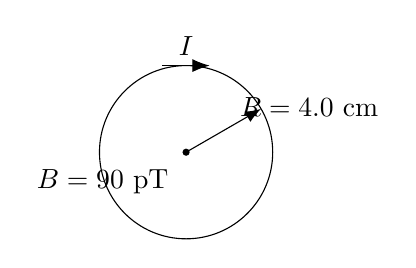
\begin{tikzpicture}[scale=1]
\draw (0,0) circle (1.1);
\fill (0,0) circle (1.3pt);
\node[below left] at (-0.1,-0.1) {$B=90$ pT};
\draw[-{Latex[length=2mm]}] (0,0) -- (30:1.1);
\node[above right] at (30:0.65) {$R=4.0$ cm};
\draw[-{Latex[length=2.2mm]}] (-0.3,1.1) -- (0.3,1.1);
\node[above] at (0,1.1) {$I$};
\end{tikzpicture}
\end{center}
The loop's radius is half the given 8.0 cm diameter, $R=4.0$ cm.}

\solve{(a)
\[
B=\frac{\mu_0I}{2R} \;\Rightarrow\; I=\frac{2BR}{\mu_0} =
\frac{2(90\times10^{-12}\text{ T})(0.040\text{ m})}{4\pi\times10^{-7}\text{
T}\cdot\text{m/A}} = \boxed{5.7\times10^{-6}\ \text{A} = 5.7\
\mu\text{A}}.
\]
(b)
\[
\mu = I\pi R^2 = (5.73\times10^{-6}\text{ A})\,\pi(0.040\text{ m})^2 =
\boxed{2.9\times10^{-8}\ \text{A}\cdot\text{m}^2}.
\]}

\review{Side by side with 29.50, the heart's dipole moment
($2.9\times10^{-8}\ \text{A}\cdot\text{m}^2$) is about $10^{30}$ times
smaller than the earth's ($8.0\times10^{22}\ \text{A}\cdot\text{m}^2$) ---
a vivid sense of just how faint biomagnetic fields are, and why detecting
them (magnetocardiography) takes extraordinarily sensitive equipment.}

%============================================================
\problem{29.61}{4}{An antiproton (same mass as a proton, but $q=-e$) moves
at 500 m/s to the left through a region with uniform fields $\vec
E=1000$ V/m (pointing up, in the plane of the page) and $\vec B=2.5$ T
(into the page). What are the magnitude and direction of the antiproton's
acceleration at this instant?}

\model{The electric and magnetic forces act simultaneously; the net force is
just their vector sum, $\vec F_{\text{net}}=q\vec E+q\vec v\times\vec B$,
and then $\vec a=\vec F_{\text{net}}/m$. Nothing here requires the two
forces to cancel --- that's a different (and more special) situation, the
one we'll meet in 29.59.}

\visualize{
\begin{center}
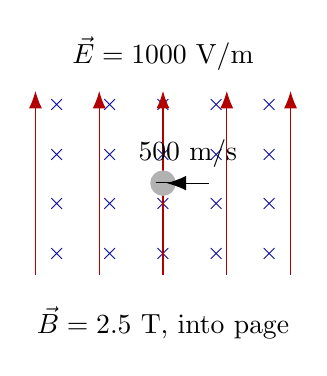
\begin{tikzpicture}[scale=0.9]
\foreach \x in {-1.5,-0.75,0,0.75,1.5}{
  \foreach \y in {-1.0,-0.3,0.4,1.1}{
    \node[blue!60!black] at (\x,\y) {\footnotesize $\times$};
  }
}
\draw[-{Latex[length=2.2mm]}, red!70!black] (-1.8,-1.3) -- (-1.8,1.3);
\draw[-{Latex[length=2.2mm]}, red!70!black] (-0.9,-1.3) -- (-0.9,1.3);
\draw[-{Latex[length=2.2mm]}, red!70!black] (0,-1.3) -- (0,1.3);
\draw[-{Latex[length=2.2mm]}, red!70!black] (0.9,-1.3) -- (0.9,1.3);
\draw[-{Latex[length=2.2mm]}, red!70!black] (1.8,-1.3) -- (1.8,1.3);
\node[above] at (0,1.45) {$\vec E=1000$ V/m};
\fill[gray!60] (0,0) circle (0.18);
\node at (0,0) {\footnotesize $-$};
\draw[-{Latex[length=2.5mm]}] (0.65,0) -- (0.05,0);
\node[above] at (0.35,0.08) {$500$ m/s};
\node[below] at (0,-1.6) {$\vec B=2.5$ T, into page};
\end{tikzpicture}
\end{center}
The antiproton is negative, so its electric force is \emph{opposite} $\vec
E$ (down), while its magnetic force, by the right-hand rule applied to a
negative charge moving left through a field into the page, works out to
point \emph{up}.}

\solve{
\[
F_E = eE = (1.60\times10^{-19}\text{ C})(1000\text{ V/m}) =
1.60\times10^{-16}\text{ N, down}
\]
\[
F_B = evB = (1.60\times10^{-19}\text{ C})(500\text{ m/s})(2.5\text{ T}) =
2.00\times10^{-16}\text{ N, up}
\]
\[
F_{\text{net}} = F_B - F_E = 0.40\times10^{-16}\text{ N, up} =
4.0\times10^{-17}\text{ N, up}
\]
\[
a = \frac{F_{\text{net}}}{m} = \frac{4.0\times10^{-17}\text{ N}}{1.67\times10^{-27}\text{
kg}} = \boxed{2.4\times10^{10}\ \text{m/s}^2\text{, up}}.
\]}

\review{The two forces are close in size (within 25\% of each other) but
don't cancel at this speed, so the antiproton still accelerates hard ---
with a proton-scale mass, even a $10^{-17}$ N force gives a $10^{10}\
\text{m/s}^2$ acceleration. 29.59 asks the reverse question: given a speed,
what field makes these two forces \emph{exactly} cancel? Same two force
expressions, just solved for a different unknown.}

%============================================================
\problem{29.59}{4}{An electron travels at $1.0\times10^7$ m/s between two
parallel plates separated by 1.0 cm and charged by a 200 V battery (top
plate positive). What magnetic field strength and direction will let the
electron pass between the plates without being deflected?}

\model{Same two force expressions as 29.61, $F_{\text{elec}}=qE$ and
$F_{\text{mag}}=qvB$ --- but now we want them to exactly cancel, so the
electron feels zero net force and travels straight through. That special
condition, $F_{\text{elec}}=F_{\text{mag}}$, is the velocity-selector
balance.}

\visualize{
\begin{center}
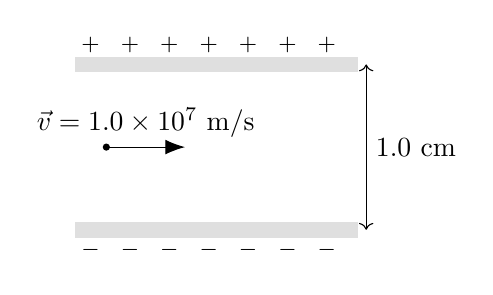
\begin{tikzpicture}[scale=1]
\fill[gray!25] (-1.8,0.95) rectangle (1.8,1.15);
\fill[gray!25] (-1.8,-1.15) rectangle (1.8,-0.95);
\foreach \x in {-1.6,-1.1,-0.6,-0.1,0.4,0.9,1.4}{
  \node at (\x,1.3) {\footnotesize $+$};
}
\foreach \x in {-1.6,-1.1,-0.6,-0.1,0.4,0.9,1.4}{
  \node at (\x,-1.3) {\footnotesize $-$};
}
\fill (-1.4,0) circle (1.3pt);
\draw[-{Latex[length=2.5mm]}] (-1.4,0) -- (-0.4,0);
\node[above] at (-0.9,0) {$\vec v=1.0\times10^7$ m/s};
\draw[<->] (1.9,-1.05) -- (1.9,1.05);
\node[right] at (1.9,0) {$1.0$ cm};
\end{tikzpicture}
\end{center}
With the top plate positive, $\vec E$ points down (toward the negative
plate). The electron, being negative, feels an electric force \emph{up}
(opposite $\vec E$), so the magnetic force needs to point \emph{down} to
cancel it.}

\solve{
\[
E = \frac{\Delta V}{d} = \frac{200\text{ V}}{0.010\text{ m}} =
2.0\times10^4\text{ V/m}
\]
\[
F_{\text{elec}} = eE = (1.60\times10^{-19}\text{ C})(2.0\times10^4\text{
V/m}) = 3.2\times10^{-15}\text{ N, up}
\]
Setting $F_{\text{mag}}=F_{\text{elec}}$ (down, to cancel the upward
electric force):
\[
evB = F_{\text{elec}} \;\Rightarrow\; B=\frac{F_{\text{elec}}}{ev} =
\frac{3.2\times10^{-15}\text{ N}}{(1.60\times10^{-19}\text{
C})(1.0\times10^7\text{ m/s})} = 2.0\times10^{-3}\text{ T}.
\]
For an electron moving right to feel a magnetic force pointing down, the
right-hand rule (flipped for the negative charge) requires $\vec B$ into the
page:
\[
\vec B = \boxed{2.0\ \text{mT, into the page}}.
\]}

\review{Check: $E/B = (2.0\times10^4\text{ V/m})/(2.0\times10^{-3}\text{
T}) = 1.0\times10^7$ m/s --- exactly the given electron speed, confirming
the balance condition $v=E/B$ (the same relation Prep 24's velocity
selector uses). Compare to 29.61: there, the fields were given numbers that
did \emph{not} satisfy $v=E/B$, so the particle accelerated instead of
passing straight through.}

%============================================================
\problem{29.65}{4}{A uniform 30 mT magnetic field points in the $+z$
direction. An electron enters the field moving at $5.0\times10^6$ m/s, at
$30^\circ$ above the $xy$-plane. Find the radius $r$ and the pitch $p$ of
the electron's spiral (helical) trajectory.}

\model{Split $\vec v$ into a component parallel to $\vec B$ and a component
perpendicular to it. The parallel component feels no magnetic force (since
$\vec v\times\vec B=0$ when they're parallel) and drifts at constant speed
along $\vec B$; the perpendicular component feels the usual magnetic force
and drives circular motion. Together they trace out a helix: $r$ comes from
the perpendicular speed, and the pitch $p$ (distance advanced per full
revolution) comes from the parallel speed times the period of that circular
motion.}

\visualize{
\begin{center}
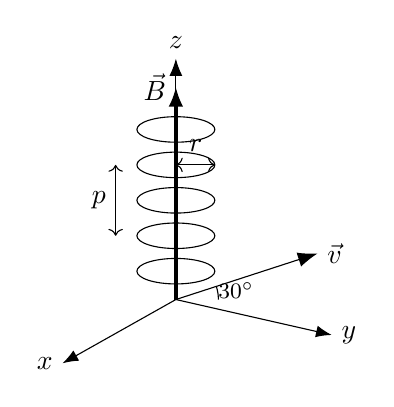
\begin{tikzpicture}[scale=0.9]
\draw[-{Latex[length=2.2mm]}] (0,0) -- (0,3.4) node[above] {$z$};
\draw[-{Latex[length=2mm]}] (0,0) -- (-1.6,-0.9) node[left] {$x$};
\draw[-{Latex[length=2mm]}] (0,0) -- (2.2,-0.5) node[right] {$y$};
\foreach \h in {0.4,0.9,1.4,1.9,2.4}{
  \draw (0,\h) ellipse (0.55 and 0.18);
}
\draw[very thick,-{Latex[length=2.5mm]}] (0,0) -- (0,3.0);
\node[left] at (0,3.0) {$\vec B$};
\draw[<->] (0,1.9) -- (0.55,1.9);
\node[above] at (0.28,1.95) {$r$};
\draw[<->] (-0.85,0.9) -- (-0.85,1.9);
\node[left] at (-0.85,1.4) {$p$};
\draw[-{Latex[length=2.5mm]}] (0,0) -- (2.0,0.65);
\node[right] at (2.0,0.65) {$\vec v$};
\draw (0.6,0) arc (0:18:0.6);
\node at (0.85,0.13) {\footnotesize $30^\circ$};
\end{tikzpicture}
\end{center}
The $30^\circ$ is measured from the $xy$-plane (not from $\vec B$), so
$v_\parallel=v\sin30^\circ$ and $v_\perp=v\cos30^\circ$.}

\solve{
\[
v_\perp = v\cos30^\circ = (5.0\times10^6\text{ m/s})(0.866) =
4.33\times10^6\text{ m/s}
\]
\[
v_\parallel = v\sin30^\circ = (5.0\times10^6\text{ m/s})(0.500) =
2.50\times10^6\text{ m/s}
\]
\[
r = \frac{mv_\perp}{eB} = \frac{(9.11\times10^{-31}\text{
kg})(4.33\times10^6\text{ m/s})}{(1.60\times10^{-19}\text{ C})(0.030\text{
T})} = \boxed{0.82\ \text{mm}}
\]
\[
T = \frac{2\pi r}{v_\perp} = \frac{2\pi(8.2\times10^{-4}\text{
m})}{4.33\times10^6\text{ m/s}} = 1.19\times10^{-9}\text{ s}
\]
\[
p = v_\parallel T = (2.50\times10^6\text{ m/s})(1.19\times10^{-9}\text{ s})
= \boxed{3.0\ \text{mm}}.
\]}

\review{As a check, the period doesn't actually need $v_\perp$ at all ---
$T=2\pi m/(eB)=2\pi(9.11\times10^{-31})/[(1.60\times10^{-19})(0.030)] =
1.19\times10^{-9}$ s, the same value, since the cyclotron period is
independent of speed. Most of the electron's speed goes into the
perpendicular, circular part of the motion ($\cos30^\circ\approx0.87$) and
less into the parallel drift ($\sin30^\circ=0.50$) --- yet the pitch
(3.0 mm) still comes out almost four times the radius (0.82 mm), since the
pitch accumulates over a \emph{full period}, not just a comparison of speed
components.}

\end{document}
